\section{Wall-function closure assessment}
\label{sec:comparative:zpg:cross-comparison}

The previous wall-resolved assessment established the discrepancy of the underlying RANS calculation from DNS. Adding a wall function to a RANS simulation introduces a further relationship between the sampled flow state and the resulting wall shear stress and heat-flux. To examine that relationship separately, the analytical closures are now evaluated on prescribed boundary layer profiles. This a-priori assessment asks how well a closure can recover the known wall heat-flux and shear stress, when its off-wall sampled inputs are ideal, i.e. supplied from the respectilve known reference boundary layer profile. It provides the comparison needed to distinguish a wall function's underlying closure behaviour from the additional changes that occur when the same wall function is coupled to full FVM CFD simulation.
\par\medskip

The detailed discussion focuses on M6Tw025 and LowH\_M3, which also carry the comparison into the subsequent coupled CFD assessment (as established in Section~\ref{subsec:comparative:zpg:case-selection}). The initial M6Tw025 sweeps use the digitally published DNS profiles and wall quantities of Zhang et al.~\cite{zhang2018direct}. LowH\_M3 lacks similar high quality published DNS reference data, so it uses the wall-resolved SA profile and its corresponding wall quantities at the matched comparison station (Section~\ref{subsec:evaluation:matching-station}) are used. For LowH\_M3, the reported closure errors are thus relative to the wall-resolved SA wall quantities. An additional M6Tw025 comparison in Section~\ref{subsec:erriso:rans-profile-influence} applies the same Li closure to DNS and resolved SA inputs to assess the influence of the supplied profile. Results for the additional cases are collected in Appendix~\ref{app:zpg:apriori}.

\subsection{A-priori inverse solution}
\label{subsec:erriso:apriori-solver}

For an a-priori assessment, a virtual sampling point is moved through a known, resolved boundary layer profile. At every sampling height, the required velocity and thermodynamic state are interpolated from that given profile and supplied to the wall-function closure equations, together with the required physical wall temperature and transport properties. The wall heat-flux and shear stress are then recovered by an inverse solution of the closure equations. The reference friction velocity defines the sampling coordinate,
\begin{equation}
    y_{\mathrm{ref}}^+
    = \frac{\rho_{w,\mathrm{ref}}u_{\tau,\mathrm{ref}}y}
    {\mu_{w,\mathrm{ref}}},
    \qquad
    u_{\tau,\mathrm{ref}}
    = \sqrt{\frac{\tau_{w,\mathrm{ref}}}{\rho_{w,\mathrm{ref}}}}.
\end{equation}

For the Li formulation, introduced in Section~\ref{subsec:wall-functions:gao-li:governing-relations}, the first-point velocity and enthalpy, the physical wall state, and an arbitrarily placed second reference state determine the generalized enthalpy--velocity relation. Two reference choices are examined. The two-point construction assumes two virtual cells of equal height, so their centres satisfy \(y_2=3y_1\). Both point states are interpolated from the resolved profile. In the alternative construction, the reference state is prescribed at the boundary layer edge. Li et al propses the former, two-point construction, so that the wall function closures are independant of the boundary layer edge quantities \cite{li2025WF}, for comparison and evaluation the latter, boundary layer edge construction was selected to be included in the analysis. In either case, the unified velocity law is inverted for \(u_\tau\), and the wall outputs follow from \(\tau_w=\rho_wu_\tau^2\) and the wall function's heat-flux relation.
\par\medskip

For the Griffin formulation, introduced in Section~\ref{subsec:wall-functions:griffin:governing-relations}, the sampled velocity and thermodynamic state are combined with the wall temperature and boundary layer-edge quantities - Griffin et al do not propose a specific approach to allow for a two-point, boundary layer edge free construction. For each sample point, the inverse-transformation model is integrated from the wall region to the sample point. The wall stress is iterated until the integrated velocity reproduces the prescribed matching point's velocity. The temperature--velocity relation then supplies the wall heat-flux. The prescribed wall stress and heat-flux of the reference profile are used to assess the recovered outputs, rather than imposed as their solution targets.
\par\medskip

Edge states are supplied according to the available reference data. Griffin uses the supplied \(\delta_{99}\) for the Zhang DNS profiles and its edge criterion for LowH\_M3, whereas the prescribed-edge Li comparison for LowH\_M3 uses the \(U=0.99U_\infty\) crossing.
\par\medskip

The reported errors in this section are signed relative differences,
\begin{equation}
    \varepsilon_X
    = 100\left(\frac{X_{\mathrm{closure}}}{X_{\mathrm{ref}}}-1\right),
    \qquad X\in\{\tau_w,q_w\}.
    \label{eq:erriso:apriori-relative-error}
\end{equation}

The reference being either the DNS wall quantities or the wall-resolved RANS quantities, depending on the profile being sampled. The a-priori assessment is therefore a standalone evaluation of the closure's ability to recover the known wall fluxes from known inputs, and thus evaluates the wall function's closure theories in isolation.

\paragraph*{Consistency with the published Griffin assessment}
An independent check of the herin implemented a-priori solver on the Griffin evaluation is available from the a-priori results of Griffin et al.~\cite[Figure~5]{griffin2023WF}. Their matching height is \(y_m=0.3\delta_{99}\). In reference wall units, this corresponds to \(y_m^+=0.3\mathrm{Re}_\tau\). Table~\ref{tab:erriso:Griffin-a-priori-validation} compares the present inverse solutions at those heights with the errors read from the published figure for two identifiable Zhang cases.

\begin{table}[H]
    \centering
    \caption[Consistency check of the Griffin a-priori solver]{Comparison of the present Griffin a-priori solver at \(y_m=0.3\delta_{99}\) with Griffin et al.~\cite[Figure~5]{griffin2023WF}. Published errors are approximate values read from the figure; the comparison checks consistency of the standalone closure evaluation.}
    \label{tab:erriso:Griffin-a-priori-validation}
    \begin{tabular}{@{}l
        S[table-format=3.3]
        S[table-format=\approx-2]
        S[table-format=-2.2]
        S[table-format=\approx-2]
        S[table-format=-2.2]@{}}
        \toprule
        & & \multicolumn{2}{c}{\(\tau_w\) error [\%]} & \multicolumn{2}{c}{\(q_w\) error [\%]} \\
        \cmidrule(lr){3-4}\cmidrule(l){5-6}
        Case & {\(y_m^+\)} & {Griffin et al.} & {Present solver} & {Griffin et al.} & {Present solver} \\
        \midrule
        M6Tw025  & 134.561 & \approx -13 & -11.56 & \approx -15 & -15.28 \\
        M14Tw018 & 192.588 & \approx -10 & -11.32 & \approx -15 & -15.91 \\
        \bottomrule
    \end{tabular}
\end{table}

The present solutions reproduce the sign and approximate magnitude of the published errors to within the uncertainties of the published graph's resolution. Their agreement supports the use of the a-priori solver used in the following to examine matching-height sensitivity of the closure theories.

\subsection{Closure errors versus sampling height}
\label{subsec:erriso:apriori-results}

Figures~\ref{fig:wall-closure:a-priori-Li-M6Tw025}--\ref{fig:wall-closure:a-priori-Griffin-LowHM3} assess the closures by Li and Griffin jointly on the M6Tw025 DNS profile and the LowH\_M3 wall-resolved SA profile. Both formulations recover the wall quantities with significant errors over the varying sampling height, but neither is notably more accurate than the other. But it shows, that the Li's two-reference-point method, rather than relying on boundary layer edge quantities, works without a systematic loss of accuracy (e.g. see Figure~\ref{fig:wall-closure:a-priori-Li-M6Tw025} dashed vs. solid line). And it should be note that both Li and Griffin's formulations don't show significantly higher errors in the buffer layer, highlighting that the blending between the sublayer and law-of-the-wall for these adaptive wall functions work well and doesn't present a \(y^+\) meshing region to be specifically avoided.
\par\medskip

Across all the investigated profiles (including the cases in Appendix~\ref{app:zpg:apriori}) Griffin gives signed shear-stress errors of approximately \(-11\%\) to \(+11\%\) and heat-flux errors of \(-14\%\) to \(+6\%\), over the reasonable range of \(1\le y_{\mathrm{ref}}^+\le100\). Over the same cases and sampling-height interval, the Li closure gives respective shear-stress errors of approximately \(-7\%\) to \(+13\%\) and heat-flux errors of \(-15\%\) to \(+18\%\). These are appreciable closure errors for prescribed, ideal, inputs and warrant ongoing research into finding better velocity transformation like by Hasan et al.\cite{hasan2023incorporating} and improved closure formulations.
\par\medskip

The heat-flux ranges exclude M2p5, whose adiabatic reference makes relative heat-flux errors undefined, and M6Tw076, owing to the reference-data limitations described in Section~\ref{sec:evaluation:benchmark-cases}.
\par\medskip

At the largest sampling height, Li's prescribed-edge M6Tw025 heat-flux error rises to approximately \(+79\%\) at \(y_1^+=400\), with a reported \(Re_\tau = 450\) \cite{zhang2018direct}, this corresponds to a sampling station at about \(0.89\delta_{99}\). Li's two-reference point method, is not applicable anymore at these sampling stations because the second reference point sits outside of the boundary layer, this is a limit of this method. The high error at these high sampling points, is consistent with increasing sensitivity of the enthalpy inversion as the sampled and reference velocities approach one another, especially because the first sampling point also lies outside the inner layer~\cite[Eq.~(40)]{li2025WF}. Griffin avoids this particular inversion sensitivity by prescribing the wall temperature--velocity slope through its Reynolds analogy. It shows significant improvement to this high \(y^+\) sensitivity, but does not establish universal validity near the boundary layer edge. The published a-priori comparison uses \(y_m=0.3\delta_{99}\); the additional WMLES matching-height studies discussed in Section~\ref{subsec:wall-functions:griffin:validation-scope} do not extend this assessment towards the edge.

\clearpage

\begin{figure}[H]
    \centering
    % Figure provenance (WSL; absolute paths):
    %   Figure: /home/mgnadlinger/OpenFOAM/mgnadlinger-v2412/src/LiWallFunctions/tests/ReverseSolver/M6Tw025_Stat_Zhang/wall_flux_errors_vs_yplus.png
    %   Python scripts:
    %     /home/mgnadlinger/OpenFOAM/mgnadlinger-v2412/src/LiWallFunctions/tests/ReverseSolver/plot_m6tw025_flux_reference_overlay.py
    %     /home/mgnadlinger/OpenFOAM/mgnadlinger-v2412/src/LiWallFunctions/tests/ReverseSolver/analyze_li_wall_function_profile_Zhang.py
    %   Data / simulation roots (high-level):
    %     /home/mgnadlinger/OpenFOAM/mgnadlinger-v2412/src/LiWallFunctions/tests/ReverseSolver/M6Tw025_Stat_Zhang
    %     /home/mgnadlinger/OpenFOAM/mgnadlinger-v2412/src/LiWallFunctions/tests/ReverseSolver/M6Tw025_Stat_Zhang_boundaryLayerEdge
    %     /home/mgnadlinger/OpenFOAM/mgnadlinger-v2412/src/LiWallFunctions/tests/ReverseSolver
    %     /home/mgnadlinger/Zhang_DNS_ZPGFP/References/Data
    %   Note: The plot combines the second-cell and boundary-layer-edge a-priori sweep directories.
    %   Note: The staged DNS input in ReverseSolver includes added Cf/Ch header fields; its DNS profile rows
    %     match References/Data.
    %   Thesis replot: Figures/Closures/plot_apriori_assessments.py; byte-for-byte
    %     saved sweeps and original paths/hashes in Figures/Closures/apriori_sources/.
    %   Layout: shear left, heat flux right; original 10.5 pt plot font retained.
    % End figure provenance.
    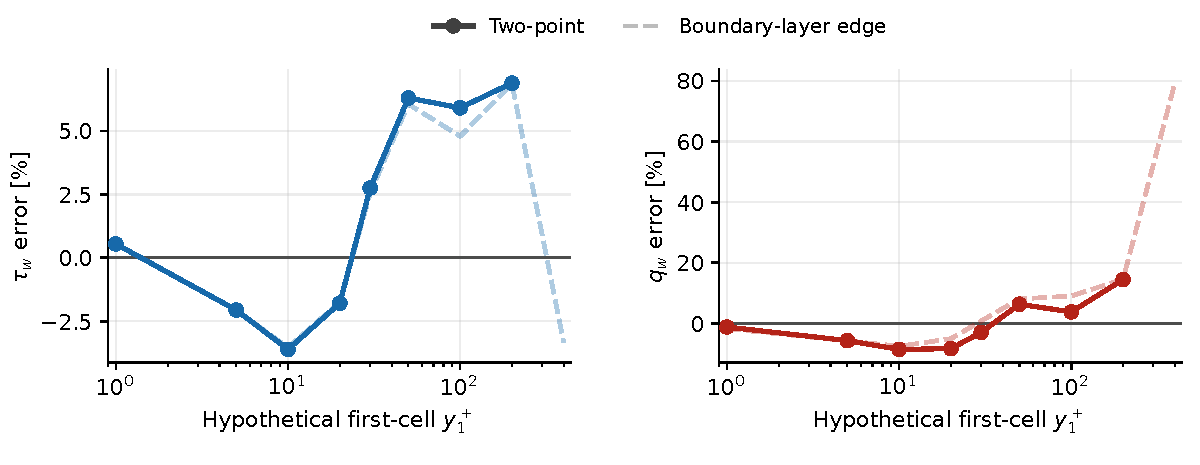
\includegraphics[width=\linewidth]{07_Error_Isolation_Results/Figures/Closures/a-priori_Li_M6Tw025.pdf}
    \caption[Li closure assessment on the M6Tw025 DNS profile]{A-priori Li wall-shear (left) and heat-flux (right) errors relative to the M6Tw025 DNS wall quantities. The solid curves use two virtual equal-height cells, with \(y_2=3y_1\); the dashed curves use a prescribed boundary layer-edge state. The horizontal coordinate is the virtual first-cell-centre height in DNS wall units. Each point is a separate inverse closure solution on the same prescribed profile.}
    \label{fig:wall-closure:a-priori-Li-M6Tw025}
\end{figure}

\begin{figure}[H]
    \centering
    % Figure provenance (WSL; absolute paths):
    %   Figure: /home/mgnadlinger/OpenFOAM/mgnadlinger-v2412/src/GriffinWallFunctions/tests/ReverseSolver/M6Tw025_Stat_Zhang/wall_flux_errors_vs_yplus.png
    %   Python script:
    %     /home/mgnadlinger/OpenFOAM/mgnadlinger-v2412/src/GriffinWallFunctions/tests/ReverseSolver/analyze_griffin_wall_function_profile_Zhang.py
    %   Data / simulation roots (high-level):
    %     /home/mgnadlinger/OpenFOAM/mgnadlinger-v2412/src/GriffinWallFunctions/tests/ReverseSolver/M6Tw025_Stat_Zhang
    %     /home/mgnadlinger/OpenFOAM/mgnadlinger-v2412/src/GriffinWallFunctions/tests/ReverseSolver
    %     /home/mgnadlinger/Zhang_DNS_ZPGFP/References/Data
    %   Note: The staged DNS input in ReverseSolver includes added Cf/Ch header fields; its DNS profile rows
    %     match References/Data.
    %   Thesis replot: Figures/Closures/plot_apriori_assessments.py; byte-for-byte
    %     saved sweeps and original paths/hashes in Figures/Closures/apriori_sources/.
    %   Layout: shear left, heat flux right; original 10.5 pt plot font retained.
    % End figure provenance.
    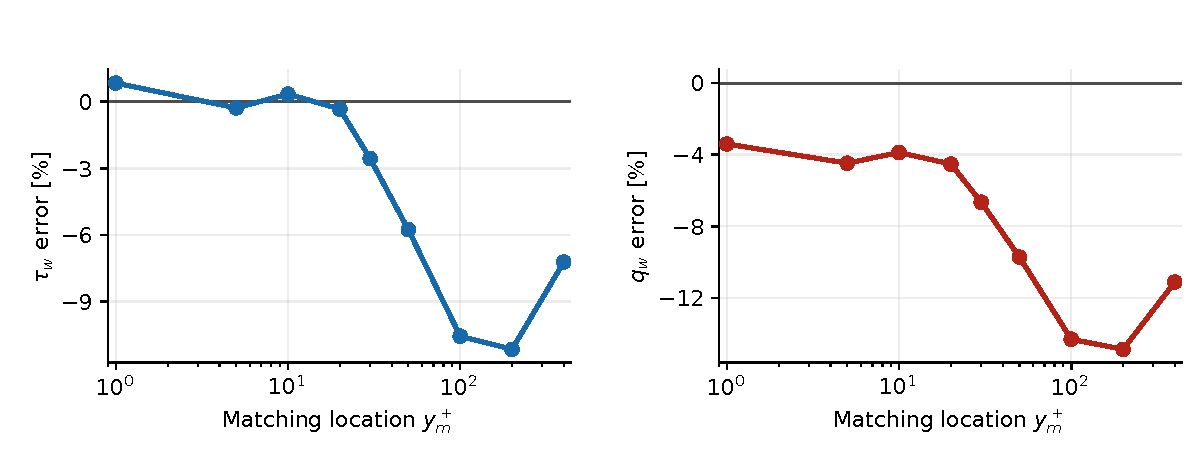
\includegraphics[width=\linewidth]{07_Error_Isolation_Results/Figures/Closures/a-priori_Griffin_M6Tw025.pdf}
    \caption[Griffin closure assessment on the M6Tw025 DNS profile]{A-priori Griffin wall-shear (left) and heat-flux (right) errors relative to the M6Tw025 DNS wall quantities. The prescribed DNS edge state remains fixed while the virtual matching height \(y_m^+\) is varied. Points above \(y_m=0.3\delta_{99}\), corresponding here to \(y_m^+\simeq134.6\), extend the assessment beyond the matching height used in the published a-priori comparison and are retained as sensitivity results.}
    \label{fig:wall-closure:a-priori-Griffin-M6Tw025}
\end{figure}

\clearpage

\begin{figure}[H]
    \centering
    % Figure provenance (WSL; absolute paths):
    %   Figure: /home/mgnadlinger/OpenFOAM/mgnadlinger-v2412/src/LiWallFunctions/tests/ReverseSolver/LowH_M3_Duan_Li/wall_flux_errors_vs_yplus.png
    %   Python scripts:
    %     /home/mgnadlinger/OpenFOAM/mgnadlinger-v2412/src/LiWallFunctions/tests/ReverseSolver/plot_m6tw025_flux_reference_overlay.py
    %     /home/mgnadlinger/OpenFOAM/mgnadlinger-v2412/src/LiWallFunctions/tests/ReverseSolver/analyze_li_wall_function_profile_Duan.py
    %   Data / simulation roots (high-level):
    %     /home/mgnadlinger/OpenFOAM/mgnadlinger-v2412/src/LiWallFunctions/tests/ReverseSolver/LowH_M3_Duan_Li
    %     /home/mgnadlinger/OpenFOAM/mgnadlinger-v2412/src/LiWallFunctions/tests/ReverseSolver/LowH_M3_Duan_Li_boundaryLayerEdge
    %     /home/mgnadlinger/OpenFOAM/mgnadlinger-v2412/src/LiWallFunctions/tests/ReverseSolver/LowH_M3_Duan
    %     /home/mgnadlinger/Duan_DNS_ZPGFP/Martin_Duan_Part4/SA_Prt0p9/LowH_M3
    %   Note: Closure input is the wall-resolved SA profile at time 20000.
    %   Note: The plot combines the second-cell and boundary-layer-edge a-priori sweep directories.
    %   Thesis replot: Figures/Closures/plot_apriori_assessments.py; byte-for-byte
    %     saved sweeps and original paths/hashes in Figures/Closures/apriori_sources/.
    %   Layout: shear left, heat flux right; original 10.5 pt plot font retained.
    % End figure provenance.
    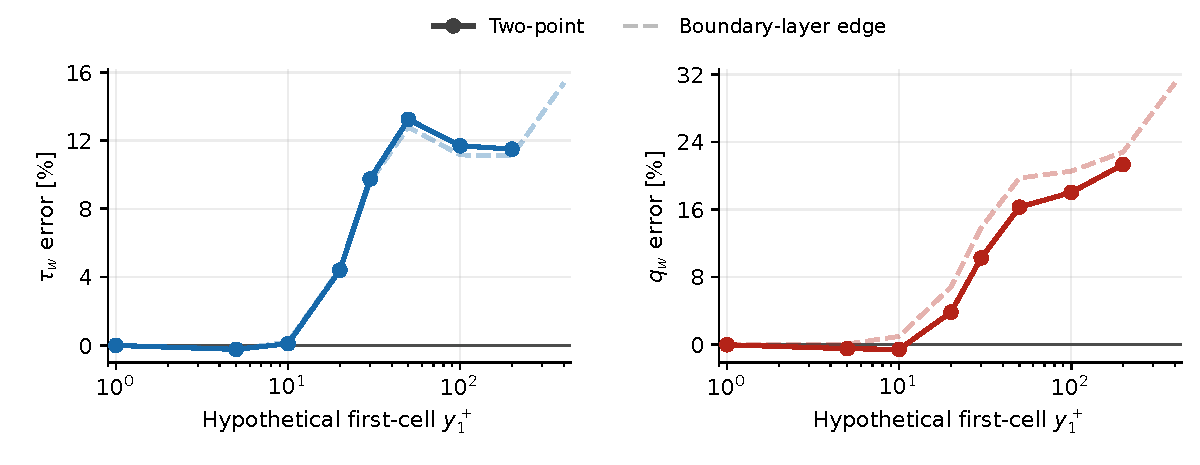
\includegraphics[width=\linewidth]{07_Error_Isolation_Results/Figures/Closures/a-priori_Li_LowHM3.pdf}
    \caption[Li closure assessment on the LowH\_M3 wall-resolved profile]{A-priori Li wall-shear (left) and heat-flux (right) errors relative to the wall-resolved SA baseline for LowH\_M3. Solid curves use the two-point formulation, with \(y_2=3y_1\), and dashed curves use the prescribed \(0.99U_\infty\) edge state. Sampling heights are expressed in wall units of the unchanged SA reference profile. These are closure errors relative to RANS, rather than errors relative to DNS.}
    \label{fig:wall-closure:a-priori-Li-LowHM3}
\end{figure}

\begin{figure}[H]
    \centering
    % Figure provenance (WSL; absolute paths):
    %   Figure: /home/mgnadlinger/OpenFOAM/mgnadlinger-v2412/src/GriffinWallFunctions/tests/ReverseSolver/LowH_M3_Duan/wall_flux_errors_vs_yplus.png
    %   Python script:
    %     /home/mgnadlinger/OpenFOAM/mgnadlinger-v2412/src/GriffinWallFunctions/tests/ReverseSolver/analyze_griffin_wall_function_profile_Duan_Part4.py
    %   Data / simulation roots (high-level):
    %     /home/mgnadlinger/OpenFOAM/mgnadlinger-v2412/src/GriffinWallFunctions/tests/ReverseSolver/LowH_M3_Duan
    %     /home/mgnadlinger/Duan_DNS_ZPGFP/Martin_Duan_Part4/SA_Prt0p9/LowH_M3
    %   Note: Closure input is the wall-resolved SA profile at time 20000.
    %   Thesis replot: Figures/Closures/plot_apriori_assessments.py; byte-for-byte
    %     saved sweeps and original paths/hashes in Figures/Closures/apriori_sources/.
    %   Layout: shear left, heat flux right; original 10.5 pt plot font retained.
    % End figure provenance.
    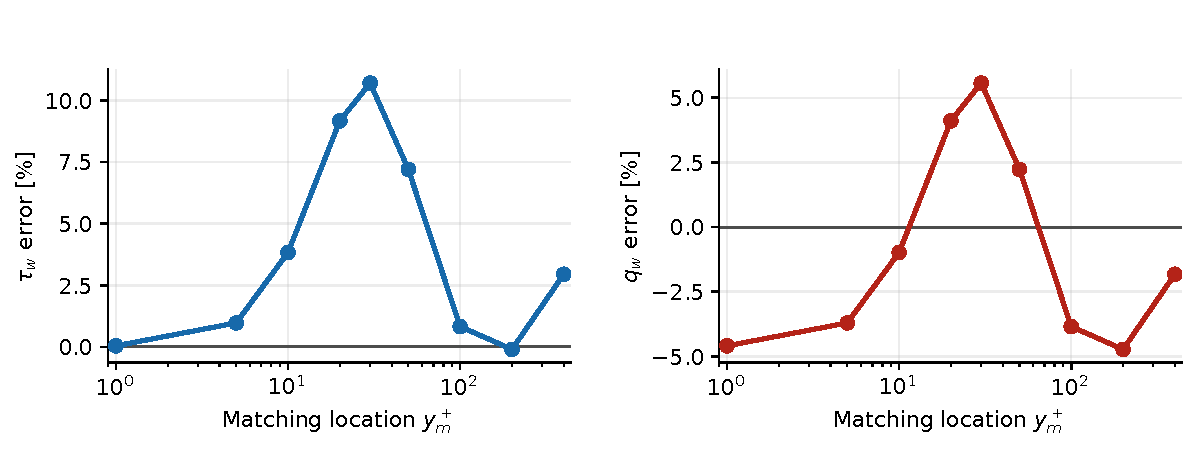
\includegraphics[width=\linewidth]{07_Error_Isolation_Results/Figures/Closures/a-priori_Griffin_LowHM3.pdf}
    \caption[Griffin closure assessment on the LowH\_M3 wall-resolved profile]{A-priori Griffin wall-shear (left) and heat-flux (right) errors relative to the wall-resolved SA baseline for LowH\_M3. The edge state is reconstructed once from the resolved profile using the Griffin boundary layer criterion, then held fixed while the virtual matching height is varied. The point at \(y_m^+=400\) lies above \(0.3\delta_{99}\) of this reconstructed boundary layer and is included as a sensitivity result.}
    \label{fig:wall-closure:a-priori-Griffin-LowHM3}
\end{figure}

\clearpage

\subsection{Influence of the prescribed RANS profile}
\label{subsec:erriso:rans-profile-influence}

In the previous Section\ref{sec:comparative:zpg:wall-resolved-baselines}, with the assessment of turbulence models, the wall-resolved M6Tw025 comparison in Figure~\ref{fig:wall-resolved:M6Tw025_BL_Profile} revealed a clear discrepancy in the temperature maximum and \(T(U)\) relation compared to the DNS reference. To quantify the consequence of this short coming of the turbulence models to the wall function closure that rely on these profiles, the Li et al. closure is evaluated on both the DNS profile and the wall-resolved SA profile at \(Pr_t=0.9\) and subsequently compared.
\par\medskip

Figure~\ref{fig:wall-closure:Li-M6Tw025-profile-influence} expresses both a-priori solved results relative to the same DNS wall quantities. Replacing the DNS profile as input, with the wall-resolved SA profile, changes the heat-flux prediction substantially, while the shear predictions remain much closer. This aligns with the SA velocity profile matching the DNS reference (see Figure~\ref{fig:wall-resolved:M6Tw025_BL_Profile} bottom right), while the \(T(U)\) profile, which feeds the wall function's energy closure, does not (see Figure~\ref{fig:wall-resolved:M6Tw025_BL_Profile} top left). At \(y_{1,\mathrm{DNS}}^+=30\), the predicted heat-flux increases by \(13.4\%\) relative to the DNS-input prediction, but shear changes by only \(0.1\%\). At \(y_{1,\mathrm{DNS}}^+=100\), the heat-flux error relative to DNS rises from \(+3.2\%\) to \(+16.0\%\). Thus, the thermal-profile discrepancy observed in the resolved calculation has a significant counterpart in the wall-function response, even where the velocity profiles appear convincing, and need to be addressed in future improvements of the turbulence models. In a fully coupled turbulence model + wall function CFD run, this error does not isolated as cleanly as in the a-priori solver here, because of the feedback of the wall function's wall quantity prediction into the overall flow field, but the underlying discrepancy still stands.

\begin{figure}[H]
    \centering
    % Figure provenance (WSL; absolute paths):
    %   Original figure: /home/mgnadlinger/OpenFOAM/mgnadlinger-v2412/src/LiWallFunctions/tests/ReverseSolver/M6Tw025_TM_closure_isolation/wall_flux_comparison.png
    %   Analysis script: /home/mgnadlinger/OpenFOAM/mgnadlinger-v2412/src/LiWallFunctions/tests/ReverseSolver/M6Tw025_TM_closure_isolation/run_comparison.py
    %   Saved data: /home/mgnadlinger/OpenFOAM/mgnadlinger-v2412/src/LiWallFunctions/tests/ReverseSolver/M6Tw025_TM_closure_isolation/comparison.csv
    %   Wall references: /home/mgnadlinger/OpenFOAM/mgnadlinger-v2412/src/LiWallFunctions/tests/ReverseSolver/M6Tw025_TM_closure_isolation/reference_states.csv
    %   Original DNS input: /home/mgnadlinger/Zhang_DNS_ZPGFP/References/Data/M6Tw025_Stat.dat
    %   Original SA input: /home/mgnadlinger/Zhang_DNS_ZPGFP/SA_Prt0p9/M6Tw025/postProcessing/TM_ZPGFP/15000/profile_Re_delta2.csv
    %   Thesis export script: thesis/07_Error_Isolation_Results/Figures/Closures/plot_tm_profile_closure.py
    %   Note: The earlier thesis PNG retained only the original figure's middle row,
    %     omitting its legend. Re-exported from saved CSVs with a shared legend;
    %     both panels retain the common DNS denominator and all eight heights.
    %   Note: Fixed omegaH=0.72; each input retains its native wall state.
    %     This is a complete-profile comparison, not a temperature-only swap.
    % End figure provenance.
    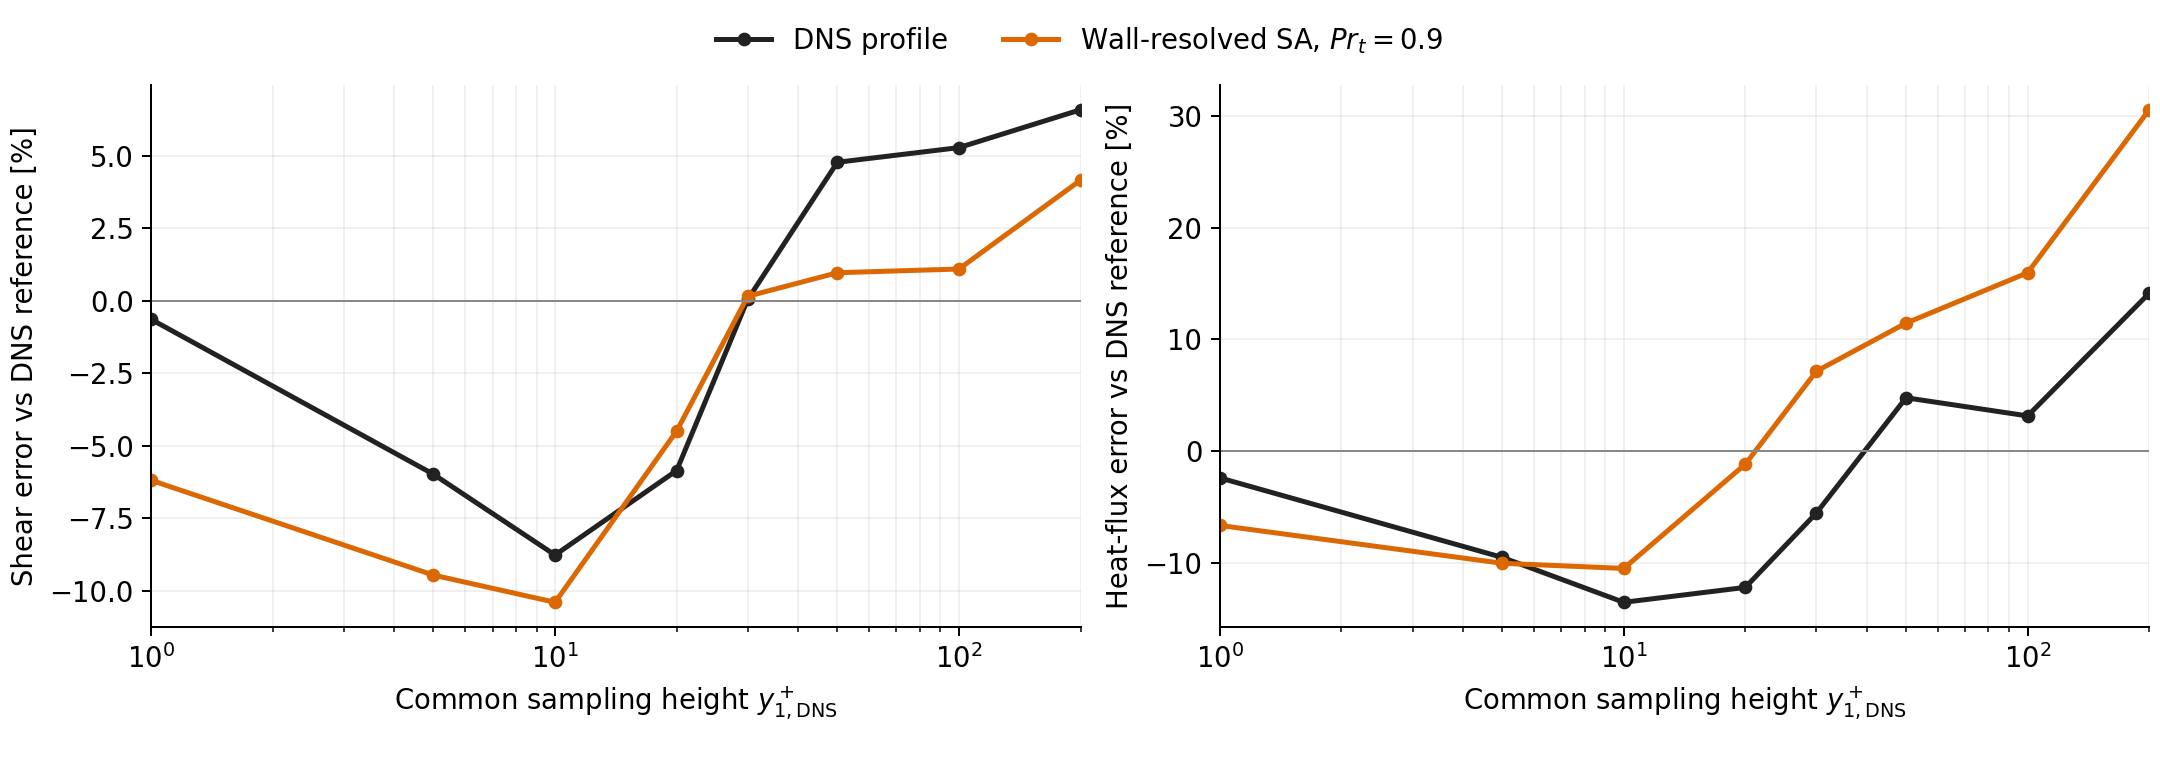
\includegraphics[width=\linewidth]{07_Error_Isolation_Results/Figures/Closures/TM_prof_err_Li-aprio.png}
    \caption[Effect of DNS and SA inputs on the M6Tw025 Li closure]{Li closure evaluated on the M6Tw025 DNS and wall-resolved SA profiles. Left: wall-shear error; right: heat-flux error. Both curves use the DNS wall heat-flux and shear stress as their reference, hence the orange line not converging to zero error at \(y_{1,\mathrm{DNS}}^+=1\). The virtual sampling heights of \(y_1\) and \(y_2=3y_1\) are identical for both inputs; the abscissa uses the supplied DNS wall units.}
    \label{fig:wall-closure:Li-M6Tw025-profile-influence}
\end{figure}

The common DNS denominator in the figure must be distinguished from recovery of each profile's own wall flux. Over e.g. the three sampled heights \(y_{1,\mathrm{DNS}}^+=30\), \(50\) and \(100\), the mean absolute heat-flux error relative to the corresponding source wall value increases from \(4.5\%\) for DNS inputs to \(17.8\%\) for SA inputs. The discrepancy is therefore more than the offset between the resolved SA and DNS wall fluxes itself, hence the discrepancy in the wall-resolved boundary layer to the DNS impacts the wall function closure's accuracy. 
\par\medskip

This is also clearly seen through the immediate mechanism, which is the inferred enthalpy--velocity wall slope in the wall function's energy closure. Li's generalized recovery enthalpy is obtained from
\begin{equation}
    h_{rg}
    =\frac{h_1-h_w(1-r)-h_Rr^2}{r(1-r)},
    \qquad r=\frac{U_1}{U_R},
    \label{eq:erriso:li-reference-inversion}
\end{equation}
where \((U_R,h_R)\) is the reference state, here the second sampling point~\cite[Eq.~(40)]{li2025WF}.

With positive heat-transfer into the cooled wall denoted by \(Q_w=|q_w|\), Li's relations give
\begin{equation}
    S=\left.\frac{\mathrm{d}h}{\mathrm{d}U}\right|_w
      =\frac{h_{rg}-h_w}{U_2},
    \qquad Q_w=\frac{\tau_w S}{Pr_w},
    \label{eq:erriso:li-profile-wall-slope}
\end{equation}
where \(h_{rg}\) follows from Equation~\eqref{eq:erriso:li-reference-inversion}~\cite[Eqs.~(40)--(41)]{li2025WF}. At \(y_{1,\mathrm{DNS}}^+=30\), changing from DNS to SA inputs raises \(S\) by \(13.3\%\), accounting for almost all of the heat-flux increase while the recovered shear is nearly unchanged because so is the sampled velocity profile. This identifies the thermal wall slope as the immediate route through which the profile mismatch affects the predicted heating. Thus future improvements to RANS turbulence models should not only improve the heat-flux and shear stress results in isolation, but also need to tackle the challenge in hypersonic cold-wall boundary layer reproducibility. 

\subsection{Summary and Implications for the coupled assessment}
The a-priori assessment (ref. Section~\ref{subsec:erriso:apriori-results}) identifies appreciable baseline errors in both closures, even when the sampled inputs are supplied from known reference profiles. However, neither formulation shows a systematic breakdown in the buffer layer. The results therefore provide no basis for excluding a buffer-layer sampling interval because of the blending between the viscous and logarithmic relations. But the remaining closure errors do warrant investigation into better, improved velocity transformations and closure theories.
\par\medskip

A comparison of supplying the a-priori solver with the DNS or the wall-resolved SA profile (ref. Section~\ref{subsec:erriso:rans-profile-influence}) identifies a further limitation: discrepancies in the wall-resolved RANS profile (as identified in Section~\ref{subsec:comparative:zpg:wr-profiles}) can substantially alter the wall-function heat-flux prediction. In the example of the Li assessment on the M6Tw025 case, it shows that a convincing velocity profile does not compensate for an inaccurate \(T(U)\) relation, which changes the inferred thermal wall slope. Improving the coupled prediction therefore requires attention to both the closure's baseline accuracy and the turbulence model's reproduction of the cold-wall thermal profile. These findings provide the context for the following assessment of the additional influence of spatial discretization in Section~\ref{subsec:comparative:zpg:yplus-sensitivity}, especially with the final isolation from the closure error by overwriting the closure theory with a fitted function in Section~\ref{subsec:comparative:zpg:fitted-closure}.
